%% Los cap'itulos inician con \chapter{T'itulo}, estos aparecen numerados y
%% se incluyen en el 'indice general.
%%
%% Recuerda que aqu'i ya puedes escribir acentos como: 'a, 'e, 'i, etc.
%% La letra n con tilde es: 'n.

\chapter{Foundations of Interest Rate Theory}
\section{Definitions and Notation}
 % the {\sl
%   objective} probability measure. The basis is assumed to carry a standard
% $q$-dimensional Wiener-Einstein process $W$, and the  
% filtration $\mathbf{F}$ is the internal one generated by $W$.
% Also assume that the measure $Q$ is a martingale measure. 

% Let $W$ be a one dimensional Wiener-Einstein stochastic process
% defined % in  a complete probability space $(\Omega, \mathcal{F},
% \mathbf{F}, P)$.  

The primary objects of our investigation are pure discount bonds, of
various maturities. All payments are assumed to be made in a fixed
currency. Moreover, we need some formal definitions.   
 
\begin{defn}[Discount Bond.] A $T-$maturity pure discount bond is a
  contract that guarantees its holder the payment of one unit of
  currency at time $T$, with no intermediate payments. The contract
  value at time $t < T$ is denoted by $P(t,T)$. Clearly, $P(T,T) = 1$
  for all 
$T$.
\end{defn}

\begin{defn}[Time to maturity.] The time to maturity $x=T-t$ is the
amount of time expressed in years from the present time $t$ to the
maturity time $T > t$. 
\end{defn}

{\sl Coupon bonds} give the owner a payment stream during the interval
$[0,T]$. These instruments have the common property, that they provide
the owner with a deterministic cash flow, and for this reason they are
also known as fixed income instruments.  

 Pure discount bond prices are the basic quantities in interest-rate
 theory, and all interest rates can be defined in terms of
 discount bond prices, as we shall see now. Therefore, they are
 often used as basic auxiliary quantities from which all rates can be
 recovered, and in turn discount bond prices can be defined in
 terms of any given family of interest rates. Notice, however, that
 interest rates are what is usually quoted in (interbank) financial
 markets, whereas zero-coupon bonds are theoretical instruments that,
 as such, are not directly observable in the market. 
In moving from discount bond prices to interest rates, and vice versa,
we need to know two fundamental features of the rates themselves: the
compounding type and the day-count convention to be applied in the
rate definition. What we mean by ``compounding type'' will be clear
from the definitions below.

\begin{defn}[Anually compounded spot interest rate.] 
The annually compounded spot interest rate prevailing at time t for
the maturity T is denoted by $Y(t,T)$ and is the constant rate at
which an investment has to be made to produce an amount of one unit of
currency at maturity, starting from $P(t,T)$ units of currency at time
$t$, when reinvesting the obtained amounts once a year. In formulas
\begin{equation}
\label{eq:ACRateDef}
Y(t,T):=P(t,T)^{-\frac{1}{T-t}}-1
\end{equation}
\end{defn}
which implies that bond prices can be expressed in terms of
annually compounded rates as
\begin{equation}
\label{eq:ZCfromACRate}
P(t,T)= \frac{1}{(1+Y(t,T))^{T-t}}
\end{equation}

\begin{defn}[Continuously compounded spot interest rate.] The
  continuously compounded spot interest rate prevailing at
  time $t$ for   the maturity $T$ is denoted by $R(t,T)$ and is the
  constant rate at which an investment of $P(t,T)$ units of currency
  at time $t$ accrues continously to yield a unit amount of currency
  at maturity $T$ 
\begin{equation}
\label{eq:CCRateDef}
R(t,T):=-\frac{\log P(t,T)}{T-t}
\end{equation}
\end{defn}
The continuously compounded interest rate is therefore a constant rate
that is consistent with the discount bond prices in that
\begin{equation}
\label{eq:CCRateAccruing}
e^{R(t,T)(T-t)} P(t,T)=1
\end{equation}
from which we can express the bond price in terms of the continuously
compounded rate $R$:
\begin{equation}
\label{eq:ZCfromCCRate}
P(t,T)= e^{-R(t,T)(T-t)} 
\end{equation}
where $T-t$, the time difference expressed in years. An
alternative to continuous compounding is simple compounding, which
applies when accruing occurs proportionally to the time of the
investment. 
\begin{defn}[Simply compounded spot interest rate.] 
 The simply \\compounded spot interest rate prevailing at time
 $t$ for the maturity T is denoted by $L(t,T)$ and is the constant
 rate at which an investment has to be made to produce an amount of
 one unit of currency at maturity, starting from $P(t,T)$ units of
 currency at time $t$, when accruing occurs proportionally to the
 investment time. 
\begin{equation}
\label{eq:SCRateDef}
L(t,T):=\frac{1-P(t,T)}{(T-t) P(t,T)}
\end{equation}
\end{defn}
We denote by $L$ such rates because the market LIBOR rates are
simply compounded. These are the most important interbank rates and
they are considered as a reference for contracts, fixing daily in
London (London InterBank Offered Rate). There exist equivalent
interbank rates fixing in other markets (e.g. the EURIBOR rate, fixing
in Brussels by the European Banking Federation). 

Suppose that we are standing at time $t$, and let us fix two other
points in time $S$ and $T$ with $t<S<T$. Let us consider now the
project of writing a forward rate agreement at time $t$ which allows
us to make an investment of one unit of currency at time $S$, and have
a {\sl deterministic} rate of return, determined at the contract time
$t$, over the interval $[ S, T]$. This agreement can be achieved with
the following replicating strategy 
\begin{enumerate}
\item At time $t$ we sell one $S$-bond. This will give us $P(t,S)$
  units of our base currency. 
\item With this money we may buy exactly a $\frac{P(t,S)}{P(t,T)}$
  amount of $T$-bonds.  
$$
P(t,S)-\frac{P(t,S)}{P(t,T)} P(t,T)=0\quad~\mathrm{in}\quad t
$$
Note that our net investment at initial time $t$ is zero.
\item At time $S$ the $S$-bond expires, so we must to pay out one
  monetary unit of our currency. 
\item At time $T$ each $T$-bond expires paying one unit of currency,
  so we will receive the payoff $P(t,S)/P(t,T)\cdot 1$. 
\item The real effect of this strategy is that, based on the contract
  agreed at $t$, for an investment of one unit of currency we have
  received in turn $P(t,S)/P(t,T)$ at time $T$. 
\end{enumerate}
Now the following crutial definition is well motivated by the
implementation of the financial strategy above. 
\begin{defn}[Simply compounded forward interest rate.]
The simple forward rate for the period $[S, T]$ contracted at $t<S<T$,
is defined as 
$$
L(t; S,T):=\frac{1}{T-S} \left( \frac{P(t,S)}{P(t,T)}-1 \right)
$$
\end{defn}
Or, in other words, the simple forward rate $L$, is the solution to
the equation 
$$
1+(T-S) L=\frac{P(t,S)}{P(t,T)}
$$
Moreover, it is straightforward to recover the spot definition making
the assignment $t=S$, i.e. the spot rates are forward when the time of
the agreement coincides with the start of the interval over which the 
interest rate is effective.

The simple forward rate $L(t;T,S)$ may be viewed as an estimate of the future spot rate $L(T,S)$.

When the maturity of the forward rate collapses towards its expiry, we have the notion
of {\sl instantaneous forward rate}. Let us consider the limit
\begin{equation}
\label{eq:instaFRDef0}
\begin{array}{rcl}
\displaystyle \lim_{\Delta T\to 0^+} L(t;T,T+\Delta T) & = &
-\displaystyle \lim_{\Delta T\to 0^+} \displaystyle \frac{P(t,T+\Delta
  T)-P(t,T)}{P(t,T+\Delta T) \Delta T}\\ 
 & = & -\displaystyle \frac{1}{P(t,T)} \frac{\partial P(t,T)}{\partial T} \\
 & = & -\displaystyle \frac{\partial \log P(t,T)}{\partial T}
\end{array}
\end{equation}

This leads to the following.

\begin{defn}[Instantaneous forward interest rate.]
The instaneous forward interest rate prevailing at time $t$ for the maturity $T>t$ is denoted by $F(t,T)$ and is defined as
\begin{equation}
F(t,T):= \displaystyle \lim_{\Delta T\to 0^+} L(t; T, T+\Delta T) = -\frac{\partial \log P(t,T)}{\partial T},
\end{equation}
so that we also have 
\begin{equation}
\label{eq:ZBfunctioninstaFR}
P(t,T)=\exp \left(-\int^T_t F(t,u) \, du \right)
\end{equation}
\end{defn}
Clearly for this notion to make sense, we need to asume smoothness of
the discount bond price function $T \mapsto P(t,T)$ for all $T$'s. 

Intuitively, the instantaneous forward rate $F(t,T)$ is a forward
interest rate at time $t$ whose maturity is very close to its expiry
$T$, say $F(t,T) \approx L(t; T, T+\Delta T)$ with $\Delta T$ small.

\section{Interest-Rate Curves}
A fundamental curve that can be obtained from the market data of
interest rates is the zero-copupon curve at a given date $t$. This
curve is the graph of the function mapping maturities into rates at
times $t$. More precisely:

\begin{defn}[Zero-rate curve.] The zero-rate curve at time $t$ is the
  graph of the function 
\begin{equation}
\label{eq:ZeroRate}
T \mapsto \left\{ 
\begin{array}{ll}
L(t,T) & t<T\leq t+1\\
Y(t,T) & T>t+1
\end{array}
\right.
\end{equation}
\end{defn}
Such a zero-coupon curve is also called the {\sl term structure of
  interest rates} (TSIR) at time $t$. By definition
(\ref{eq:ZeroRate}), it is a plot at time $t$ of simply-compounded
interest rates for all maturities $T$ up to one year and of
annually-compounded rates for maturities $T$ larger than one year.  
\begin{figure}[!h]
\centering
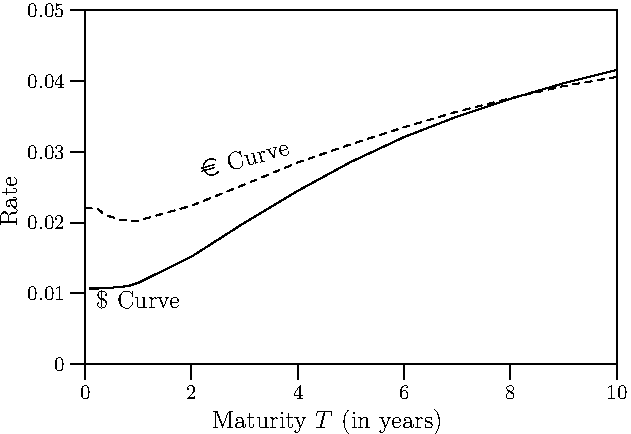
\includegraphics{Ch1Figure1.pdf}
\caption{Zero-rate curves on July 1, 2003. The normal line
  corresponds to US dollar rates and the dashed one to the euro
  rates.\label{fig:ZRCurves}}
\end{figure}
Recall that at times it may be considered the sample for rates with
different compounding conventions, such as for example  
$$
T \mapsto R(t,T), \quad T>t
$$
\begin{defn}[Discount bond curve.] The Discount bond curve at time $t$
  is the graph of the function 
\begin{equation}
\label{eq:ZeroBond}
T \mapsto P(t,T),\quad T>t
\end{equation}
\end{defn}
which, because of the positivity of interest rates, is a
$T$-decreasing function starting from $P(t,t)=1$. Two examples of such
a curve ara shown in \ref{fig:DiscCurve}
\begin{figure}[!h]
\centering
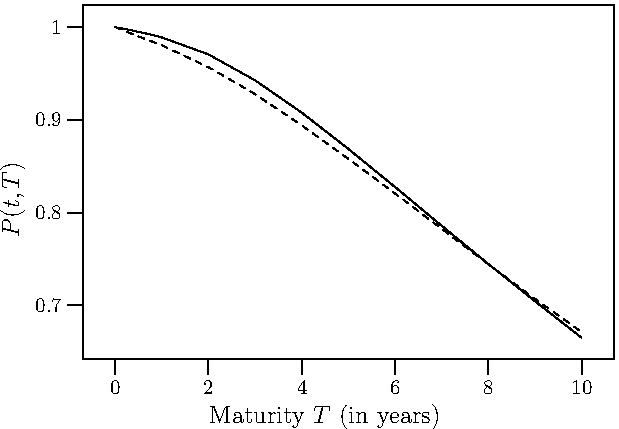
\includegraphics{Ch1Figure2.pdf}
\caption{Term structure of discount bonds on July 1, 2003. The
  normal line belongs to the US dollar discount bond curve and the
  dashed one to the euro.\label{fig:DiscCurve}}   
\end{figure}

\subsection{The Short Rate and the Money-Market Account}
\begin{defn}[Short rate.]
The instantaneous spot interest rate, also referred as the short rate,
is the continuously-compounded insterest rate when time to maturity
collapses to zero: 
\begin{equation}
\label{eq:SRLimitDef}
r(t)=\lim_{\Delta t \to 0} R(t,t+\Delta t)
\end{equation}
\end{defn}
Let us work out this limit
\begin{equation}
\label{eq:SRForwrdDef}
\begin{array}{rcl}
\displaystyle \lim_{\Delta t\to 0} R(t,t+\Delta t) & = &
-\displaystyle \lim_{\Delta t\to 0} \displaystyle \frac{\log
  P(t,t+\Delta t)}{(t+\Delta t)-t} \\  
 & = & -\displaystyle \lim_{\Delta t\to 0} \frac{\log P(t,t+\Delta
   t)-\log P(t,t)}{(t+\Delta t)-t} \\
 & = & -\displaystyle \left. \frac{\partial \log P(t,\theta)}{\partial
     \theta} \right|_{\theta=t} \\
 & = & F(t,t)
\end{array}
\end{equation}
The next definition we consider is the definition of a money-market
account. A money-market account represents a locally riskless
investment, where profit is accrued continuously at the short rate
prevailing in the market at every instant.  

\begin{defn}[Money-market account.] We define $B(t)$ to be the value
  of a money-market account at time $t\geq 0$. Assume that $B(0)=1$,
  and that the money-market account evolves according to the following
  differential equation: 
\begin{equation}
\label{eq:RiskFreeAsset}
dB(t)=r(t) B(t) dt,\qquad B(0)=1,
\end{equation}
where $r(t)$ is a positive stochastic process, i.e.,
\begin{equation}
\label{eq:DepofunctioninstaShortRate}
B(t)=\exp\left( \int_0^t r(s)\, ds\right).
\end{equation}
\end{defn}

\section{A Brief Note on Martingale Modeling}
Throughout this work we consider a continuous trading economy, with a
finite trading interval given by $[0,\Theta]$. The uncertainty is
modelled by the filtered probability space $(\Omega, \mathcal{F},
\mathbf{F}, \mathbb{P})$ where $\Omega$ denotes a sample space, with elements
$\omega\in\Omega$; $\mathcal{F}$ denotes a $\sigma$-algebra on
$\Omega$; and $\mathbb{P}$ denotes a probability measure in $(\Omega,
\mathcal{F})$. The uncertainty is resolved over $[0, \Theta]$
according to the filtration $\mathbf{F}=\{\mathcal{F}_t \}_{t \geq
  0}$. 

We consider a financial market $S=[~S_0~S_1~\dots~S_n~]^T$ with a
riskless investment, $S_0$, or money market account given by
(\ref{eq:RiskFreeAsset}), and $n$ risky assets which all follow It\^o
processes driven by a $q$-dimensional Wiener-Einstein process, $W$,
$$ 
dS_i=S_i( \mu_i dt + \sigma_i \cdot dW),\quad S_i(0)>0,\quad i=1,\dots,n.
$$
the appreciation rates $\mu_i$ and the volatility row vectors
$\sigma_i=[~\sigma_{i1}~\dots~\sigma_{iq}~]$ are assumed to be 
$\mathcal{F}_t$-adapted, intuitively, this means that they all depend on
past values but not on future. They also satisfy the integrability
conditions 
\begin{equation}
\label{eq:Regularity}
\int_0^\Theta |\mu_i| dt<\infty,\; \int_0^\Theta ||\sigma_i||^2
dt<\infty \quad i=1,\dots,n 
\end{equation}
almost surely.

A continuous time {\sl trading strategy} is any $\mathbb{R}^{n+1}$-valued
$\mathcal{F}_t$-adapted stochastic process 
$$
\phi(t)=[~\phi_0(t)~\dots~\phi_n(t)~]
$$
where $\phi_i(t)$ denotes the holdings in the asset $i$ at time
$t$. The asset holdings $\phi_i(t)$ are furthermore assumed to satisfy
similar regularity conditions as the presented in 
(\ref{eq:Regularity}).

Its corresponding {\sl value process} is
$$
V(\phi,t)=\phi (t)\cdot S(t)=\sum^n_{i=0} \phi_i(t) S_i(t)
$$

The {\sl portfolio} or trading strategy $\phi$, is called {\sl
  self-financing} when
\begin{equation}
\label{eq:SelfFinancing}
V(\phi,t)=V(\phi,0)+\sum_{i=0}^n\int_0^t \phi_i(s) dS_i(s),\quad
t\in[0, \Theta],
\end{equation}
where $\int \phi_i(s) dS_i(s)$ denote It\^o integrals. Hence, a
self-financing trading strategy is a trading strategy that requires
nor generates funds between time $0$ and time $\Theta$.

\subsection{Martingale Measures, Derivative Securities and Arbitrage}
All prices above are interpreted as being given in terms of some a
priori given {\sl numeraire}, or monetary basis. Tipically this {\sl
  numeraire} is the domestic currency like \euro, but we may, of
course, equally express all prices denominated in some other {\sl
  numeraire}. In fact, any asset which has strictly positive prices
for all $t\in [0, \Theta]$ is a {\sl numeraire}.

Suppose that, for some $p\leq n$, the $p$-asset is a {\sl numeraire}
. The prices of other assets $i\neq p$ denominated in $S_p$ are called
the {\sl relative prices} or {\sl discounted prices} and we denote
them by 
$$
\widetilde{S}_i:=S_i/S_p.
$$
We denote the {\sl relative value process} as well by
$$
\widetilde{V}:=\frac{V}{S_p}=\sum_{i\neq p}^n \phi_i \widetilde{S}_i 
$$
Let $(\Omega, \mathcal{F}, \mathbb{P} )$ denote the probability space
from the beginning of this section. Consider now the set that contains
all probability measures $\mathbb{Q}^*$ such that:
\begin{enumerate}
\item $\mathbb{Q}^* \sim \mathbb{P}$, i.e. both measures have the same
  null-sets; 
\item the relative processes $\widetilde{S}_i$ are martingales under
  $\mathbb{Q}^*$ for all $i$, i.e. for $t\leq s$
$$
\widetilde{S}_i(t)=\mathbb{E}^{\mathbb{Q}^*}[ \widetilde{S}_i(s)|\mathcal{F}_t].
$$
\end{enumerate}
The measures $\mathbb{Q}^*$ are called {\sl equivalent martingale
  measures}. Suppose we pick one particular equivalent martingale
measure
$\mathbb{Q}^*$. 
\begin{defn}[Derivative security.] Is any $\mathcal{F}_t$-measurable
  random variable $h(T)$ such that
$$
\mathbb{E}^*(|h(T)|) < \infty,
$$
where $\mathbb{E}^*$ denotes expectation under the equivalent martingale
measure $\mathbb{Q}^*$. 
\end{defn}
Hence, derivative securities are those assets for which the
expectation of the payoff is well defined. If we can find a
self-financing trading strategy $\phi$ such that
$\widetilde{V}(\phi,T)=h(T)$ with probability one, the derivative is
said to be {\sl attainable}. The self-financing trading strategy is
then called a {\sl replicating strategy}. If in an economy \emph{all}
derivative securities are attainable, the economy is called {\sl
  complete}.

An {\sl arbitrage portfolio} is a self-financing trading strategy
$\phi$, with 
$$\mathbb{P}[\widetilde{V}(\phi,T)\geq 0]=1, \quad\textrm{with}\quad
\widetilde{V}(\phi,0)<0,  
$$ 
thus, an arbitrage trading strategy is capable to produce a ``free
lunch'', because with initial negative costs we obtain at terminal 
time a non-negative value of the portfolio denominated in the chosen
numeraire.
\begin{tma}[Unique Equivalent Martingale Measure.] 
A continuous trading economy is free of arbitrage trading strategies
and every derivative security is attainable, i.e. the market is
complete, if for every choice of numeraire there exists a unique
martingale measure.
\end{tma}
\begin{demo}
See \cite{HaKreps:1978}. 
\end{demo}

Thus for a given numeraire $M$ with unique martingale measure
$\mathbb{Q}^M$, the value of a self-financing trading strategy
$$
\widetilde{V}(\phi,t)=\frac{V(\phi,t)}{M(t)}
$$
is a $\mathbb{Q}^M$-martingale. Hence, for a replicating strategy
$\phi_h$ that replicates the derivative security $h(T)$ we obtain
$$
\mathbb{E}^M \left[\frac{h(T)}{M(T)}\Big|\mathcal{F}_t \right]=
\mathbb{E}^M\left[\frac{V(\phi_h,T)}{M(T)}\Big|\mathcal{F}_t\right]= 
\frac{V(\phi_h,t)}{M(t)}
$$
where the last equality follows from the definition of a
martingale. Combining the first and the last expression yields
\begin{equation}
\label{eq:FundEqAssetPricing}
V(\phi_h, t)=M(t)\mathbb{E}^M\left[
  \frac{h(T)}{M(T)}\Big|\mathcal{F}_t\right]  
\end{equation}
This formula can be used to determine the value at time $t<T$ for any
derivative security $h(T)$. In particular, absence of arbitrage and
market completeness implies the existence of the unique probability
measure $\mathbb{Q}^B$, equivalent to the physical $\mathbb{P}$, under
which the price of any discount bond or $T$-bond, appropiately
discounted by the money-market account $S_0(t)=B(t)$, is a
$\mathbb{Q}^B$-martingale. 
$$
\widetilde{P}(t,T):=\frac{P(t,T)}{B(t)}=\mathbb{E}^B\left[
  \frac{P(T,T)}{B(T)}\Big|\mathcal{F}_t\right]=\mathbb{E}^B \left[ 
  e^{-\int_0^T r(u) du}P(T,T)\bigg|\mathcal{F}_t\right] 
$$
Combining this fact with the fact that a $T$-bond is a derivative
security which has price $1$ at its maturity we can write the
well-known {\sl arbitrage-free pricing} formula 
\begin{equation} 
\label{ArbitrageFree}
P(t,T)=\mathbb{E}^{B} \left[  e^{-\int_t^T r(s) ds} \bigg| \mathcal{F}_t \right],
\end{equation}
where we have used that $B(t)$ is $\mathcal{F}_t$-measurable. Let us
now introduce a convenient definition.\newpage \begin{defn}[Stochastic discount factor.] The stochastic discount
  factor $D(t,T)$ is given by
\begin{equation}
D(t,T)=\frac{B(t)}{B(T)}=\exp\left(-\int_t^T r(u)\: du\right)
\end{equation}
\end{defn}
\newpage\mbox{}\thispagestyle{empty}
